\documentclass[a4paper,14pt]{extreport}
\usepackage[left=1.5cm,right=1.5cm,
    top=1.5cm,bottom=2cm,bindingoffset=0cm]{geometry}
\usepackage{scrextend}
\usepackage[T1,T2A]{fontenc}
\usepackage[utf8]{inputenc}
\usepackage[russian,ukrainian,english]{babel}
\usepackage{tabularx}
\usepackage{amssymb}
\usepackage{color}
\usepackage{amsmath}
\usepackage{mathrsfs}
\usepackage{listings}
\usepackage{graphicx}
\graphicspath{ {./images/} }
\usepackage{lipsum}
\usepackage{xcolor}
\usepackage{hyperref}
\usepackage{tcolorbox}
\usepackage{tikz}
\usepackage[framemethod=TikZ]{mdframed}
\usepackage{wrapfig,boxedminipage,lipsum}
\mdfdefinestyle{MyFrame}{%
linecolor=blue,outerlinewidth=2pt,roundcorner=20pt,innertopmargin=\baselineskip,innerbottommargin=\baselineskip,innerrightmargin=20pt,innerleftmargin=20pt,backgroundcolor=gray!50!white}
 \usepackage{csvsimple}
 \usepackage{supertabular}
\usepackage{pdflscape}
\usepackage{fancyvrb}
%\usepackage{comment}
\usepackage{array,tabularx}
\usepackage{colortbl}

\usepackage{varwidth}
\tcbuselibrary{skins}
\usepackage{fancybox}


\usepackage{tikz}
\usepackage[framemethod=TikZ]{mdframed}
\usepackage{xcolor}
\usetikzlibrary{calc}
\makeatletter
\newlength{\mylength}
\xdef\CircleFactor{1.1}
\setlength\mylength{\dimexpr\f@size pt}
\newsavebox{\mybox}
\newcommand*\circled[2][draw=blue]{\savebox\mybox{\vbox{\vphantom{WL1/}#1}}\setlength\mylength{\dimexpr\CircleFactor\dimexpr\ht\mybox+\dp\mybox\relax\relax}\tikzset{mystyle/.style={circle,#1,minimum height={\mylength}}}
\tikz[baseline=(char.base)]
\node[mystyle] (char) {#2};}
\makeatother

\definecolor{ggreen}{rgb}{0.4,1,0}
\definecolor{rred}{rgb}{1,0.1,0.1}
\definecolor{amber}{rgb}{1.0, 0.75, 0.0}
\definecolor{babyblue}{rgb}{0.54, 0.81, 0.94}
\definecolor{asparagus}{rgb}{0.53, 0.66, 0.42}
\definecolor{chartreuse}{rgb}{0.5, 1.0, 0.0}
\definecolor{darkorchid}{rgb}{0.6, 0.2, 0.8}

\usepackage{float}
\usepackage{wrapfig}
\usepackage{framed}
%for nice Code{
\lstdefinestyle{customc}{
  belowcaptionskip=1\baselineskip,
  breaklines=true,
  frame=L,
  xleftmargin=\parindent,
  language=C,
  showstringspaces=false,
  basicstyle=\small\ttfamily,
  keywordstyle=\bfseries\color{green!40!black},
  commentstyle=\itshape\color{purple!40!black},
  identifierstyle=\color{blue},
  stringstyle=\color{orange},
}
\lstset{escapechar=@,style=customc}
%}


\begin{document}
\pagecolor{white}

%----------------------------------------1
\newtcbox{\xmybox}[1][red]{on line, arc=7pt,colback=#1!10!white,colframe=#1!50!black, before upper={\rule[3pt] {0pt}{10pt}},boxrule=1pt,boxsep=0pt,left=6pt,right=6pt,top=2pt,bottom=2pt}

\begin{center}\xmybox[green]{Mnatsakanov Anton} \xmybox[amber]{DP-82} \xmybox[blue]{Variant №5}
\vspace{1cm}

\end{center}


\begin{center}У чому полягає модель Дебая для опису теплоємності?\end{center}

In short, the physical quantity $ \hbar \omega_D $ is called the Debye energy, it is compared to the thermal energy $ k_BT $ at some temperature called the Debye temperature,
denoted as $ \theta_D $. Thus, $ \hbar \omega_D = k_B \theta_D $, $ \Rightarrow $ $ \theta_D = \dfrac {\hbar \omega_D} {k_B} $. Thus, the crystal in question
crystal is characterized by both the Debye frequency of elastic oscillations $ \omega_D = 2 \pi \upsilon_D $ and the Debye temperature $ \theta_D $ characteristic of the same crystal,
are related to each other via the fundamental constants Planck's constant $\hbar $ and Boltzmann's constant $ k_B $. Therefore, theorists often estimate the temperature in
in units of "frequency" and frequency in units of "temperature". \\


To explain the effect of the bonding of atoms on the frequencies of their vibrations, Fig. 1, a shows two models - free and bound pendulums. For a free pendulum, the natural frequency of oscillation $ \omega $ depends only on its length - this pendulum mimics the independent oscillator models discussed above.
This situation is compared to two elastically coupled pendulums whose oscillatory process is already more complex: each of them has the same natural frequency $ \omega $, but an additional Raman frequency $ \Omega $ also appears. If there were three pendulums, there would be three characteristic frequencies for such a system. Obviously, for n pendulums (imitating a crystal lattice with n atoms) the characteristic frequencies of vibrations would be n + 1 already.\\
\begin{figure}[h]
\center{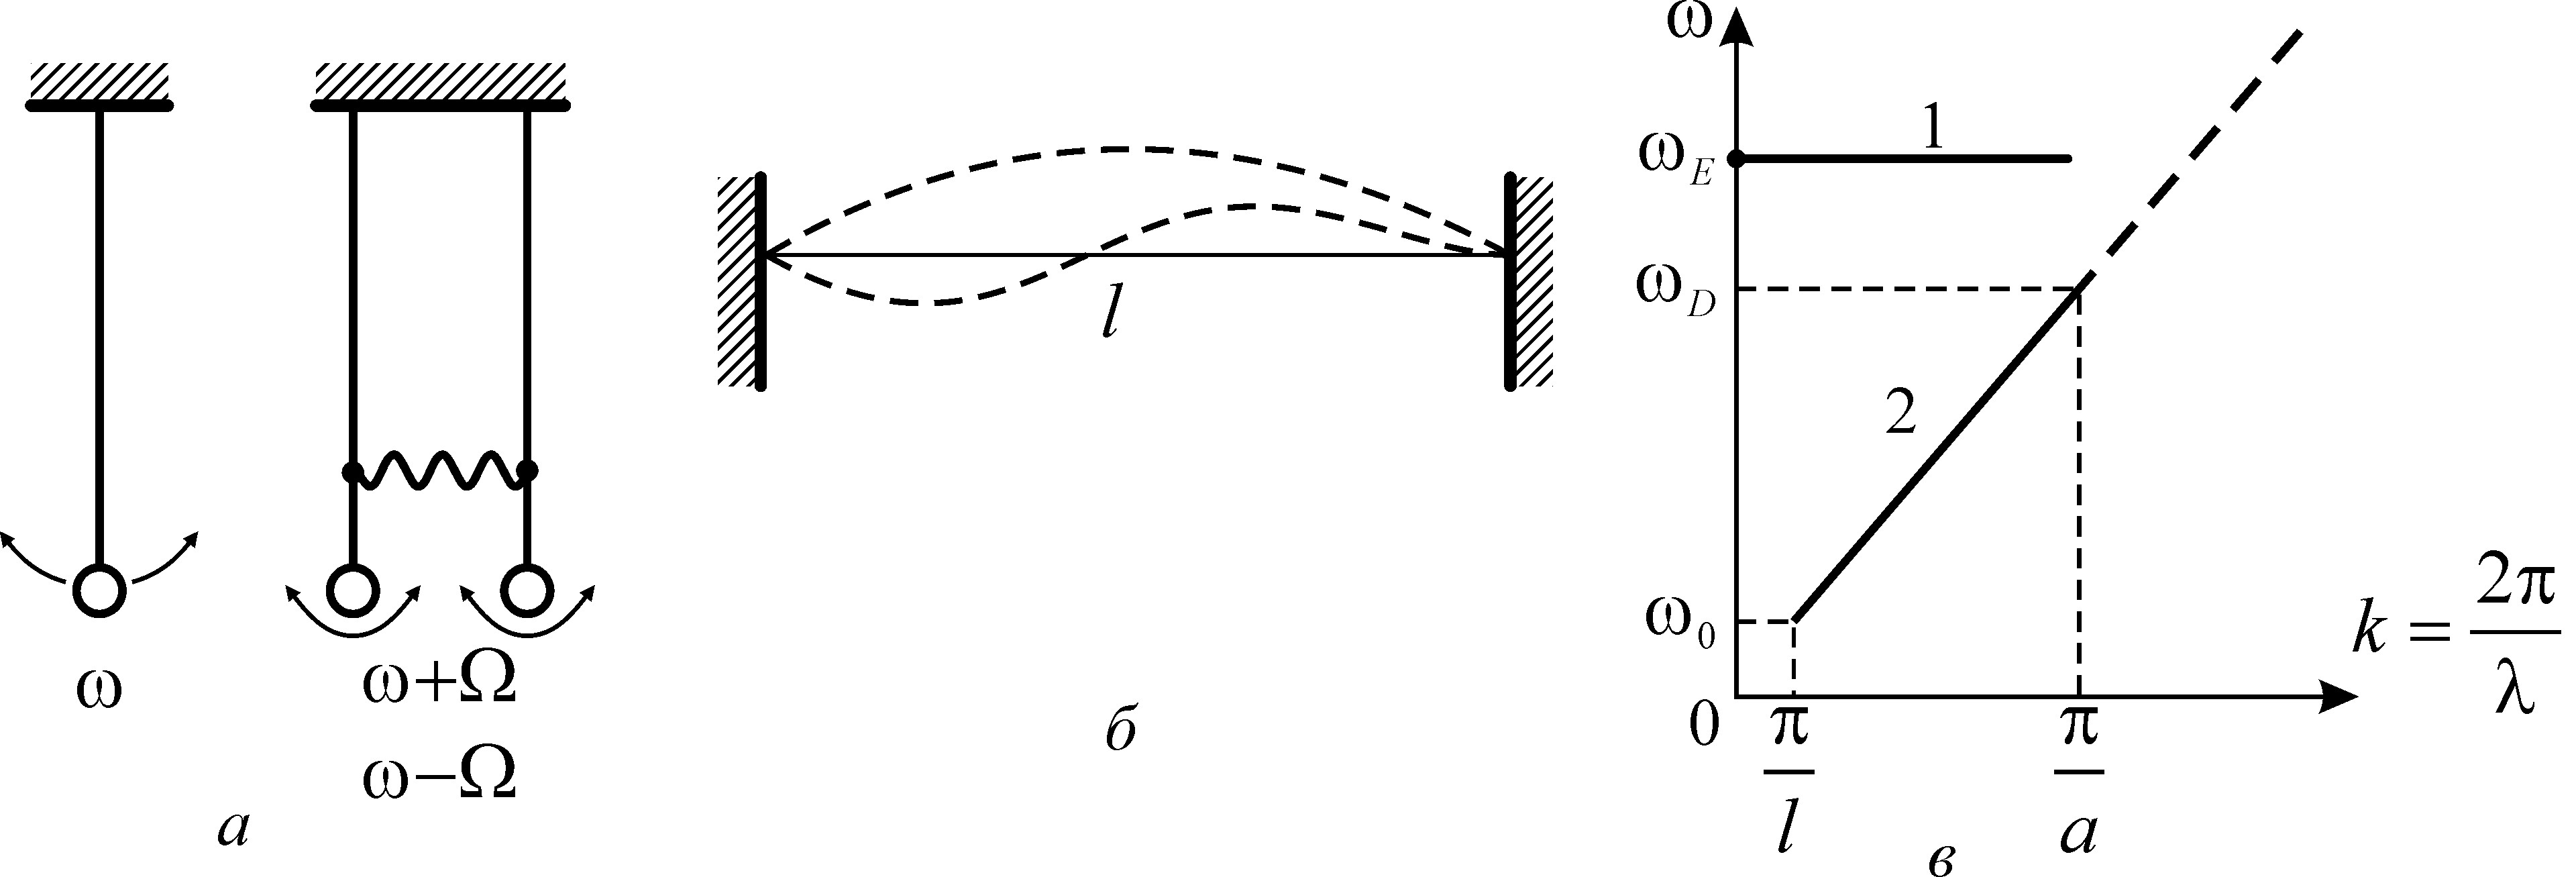
\includegraphics[width=0.7\linewidth]{1.png}}
\caption{Explanations of the Debye model: a - single and two coupled pendulums, b - oscillations of a string - the basic tone and the first overtone, c - dependence of the oscillation frequency of the string on its length, showing both the $ \omega_E $ frequency of the un coupled oscillator (1), and the dependence $ \omega (k) $ for coupled oscillators (2) with the maximum frequency $ \omega_D $}
\label{ris1}
\end{figure}












The Debye model considers the motion of the centers of mass of the N elements of the lattice connected with each other. This complex motion (lattice vibrations) is considered equivalent to the motion of 3N one-dimensional harmonic oscillators. The coordinates of these harmonic oscillators are called normal coordinates, and their oscillations are called normal vibrations.
The internal energy and heat capacity of a solid body consist of additive contributions of individual normal oscillations. To derive a formula describing the dependence of heat capacity on temperature, it is necessary to know the frequency spectrum of normal vibrations. This spectrum can be calculated theoretically: in the case of a simple lattice, the solution contains three frequency (acoustic) branches of the dependence $ \omega $ (k), which correspond to three possible independent orientations of the polarization vector of the lattice waves, that is three types of elastic waves raised in the lattice (two transverse and one longitudinal). \\

At high temperatures, all normal lattice vibrations are already excited, and therefore a further increase in temperature can no longer lead to an increase in their number. As a result, at high temperatures the energy of the solid can increase only by increasing the degree of excitation of normal vibrations, causes the increase in their average energy kT linearly with T, and the change in the energy of the body as a whole should be proportional to T: $$ E _ {\text {december}} ~ T $$

For most solids, the Debye temperature does not exceed the "normal" temperature, that is, $\theta_D $ <300 K (usually $\theta_D $ is less than room temperature). Therefore, almost all solids under normal conditions (200 $ ^ \circ $ C) do not exhibit quantum features. However, there are important exceptions for practice (diamond, beryllium oxide, magnesium oxide, etc.), for which the Debye temperature is anomalously high (over 1000 K). Such crystals, even as dielectrics, have a very high thermal conductivity under normal conditions and are therefore important for electronic applications. In the case of low temperatures the main contribution to the vibrational energy of the crystal is made by long acoustic waves. The energy of the oscillators corresponding to them is small and therefore they are easily excited. Short acoustic waves and optical waves are practically not excited at low temperatures: there is not enough thermal energy to break them when the temperature T <$ \theta_D $.\\

Debye's theory agrees very well with experiment. It should be noted that the Debye temperature characterizes not only the heat capacity, but also other properties of a solid (thermal conductivity, thermal expansion, melting point, elastic properties, etc.).

\end{document}
